\subsection{Performance Evaluation}
\label{sec:evaluation}
We have compared the processing time of each user login in UPRESSO, with the original OIDC implementation (MITREid Connect) and SPRESSO which only hides the user's accessed RPs from IdP.

%(with 4 cores, 8 threads)\
%\noindent{\textbf{Configuration.}} 
We run the evaluation on 3 physical machines connected in a separated 1Gbps network. A DELL OptiPlex 9020 PC (Intel Core i7-4770 CPU, 3.4GHz, 500GB SSD and 8GB RAM) with Window 10 prox64 works as the IdP. A ThinkCentre M9350z-D109 PC (Intel Core i7-4770s CPU, 3.1GHz, 128GB SSD and 8GB RAM) with  Window 10 prox64 servers as RP. The user adopts Chrome v75.0.3770.100 as the user agent on the Acer VN7-591G-51SS Laptop (Intel Core i5-4210H CPU, 2.9GHz, 128GB SSD and 8GB RAM) with  Windows 10 prox64. For SPRESSO, the extra trusted entity FWD is deployed on the same machine as IdP. The monitor demonstrates that  the calculation and network processing of the IdP does not become a bottleneck.

%\noindent{\textbf{Performance.}} 
We have measured the processing time for $1000$ login flows, and the the results is demonstrated in Figure~\ref{fig:evaluation}. The average time is 208 ms, 113 ms and 308 ms for UPRESSO, MITREid Connect and SPRESSO respectively.


For better comparison, we further divide a SSO login flow into 4 phases, which : 1. \textbf{Authentication request initiation} (Steps 1-2.5 in Figure~\ref{fig:process}), the period which starts before the user sends the login request and ends after the user receive the identity proof request transmitted from itself.
%IdP has received the identity proof request;
2. \textbf{Identity proof generation} (Step 4 in Figure~\ref{fig:process}), denoting the construction of identity proof at the IdP (excluding the user authentication); 3. \textbf{Identity proof transmition} (Steps 5.1-5.3 in Figure~\ref{fig:process}), for transmitting the proof from the IdP to the RP with the user's help; and 4. \textbf{Identity proof verification} (Steps 6 in Figure~\ref{fig:process}), for the RP  verifying and parsing the proof for the user's $Account$. 
%However, the HTTP transmission is consisted of the pairwise request and response, so that in the implementation of timer, the step 14 and 19 are counted as the identity proof transmitting. To avoid the time difference in each computer, we consistently anchor the time point at user agent where the time is always achieved from the user's PC. The detailed comparison is shown in Figure~\ref{fig:evaluation}.



\begin{figure}
  \centering
  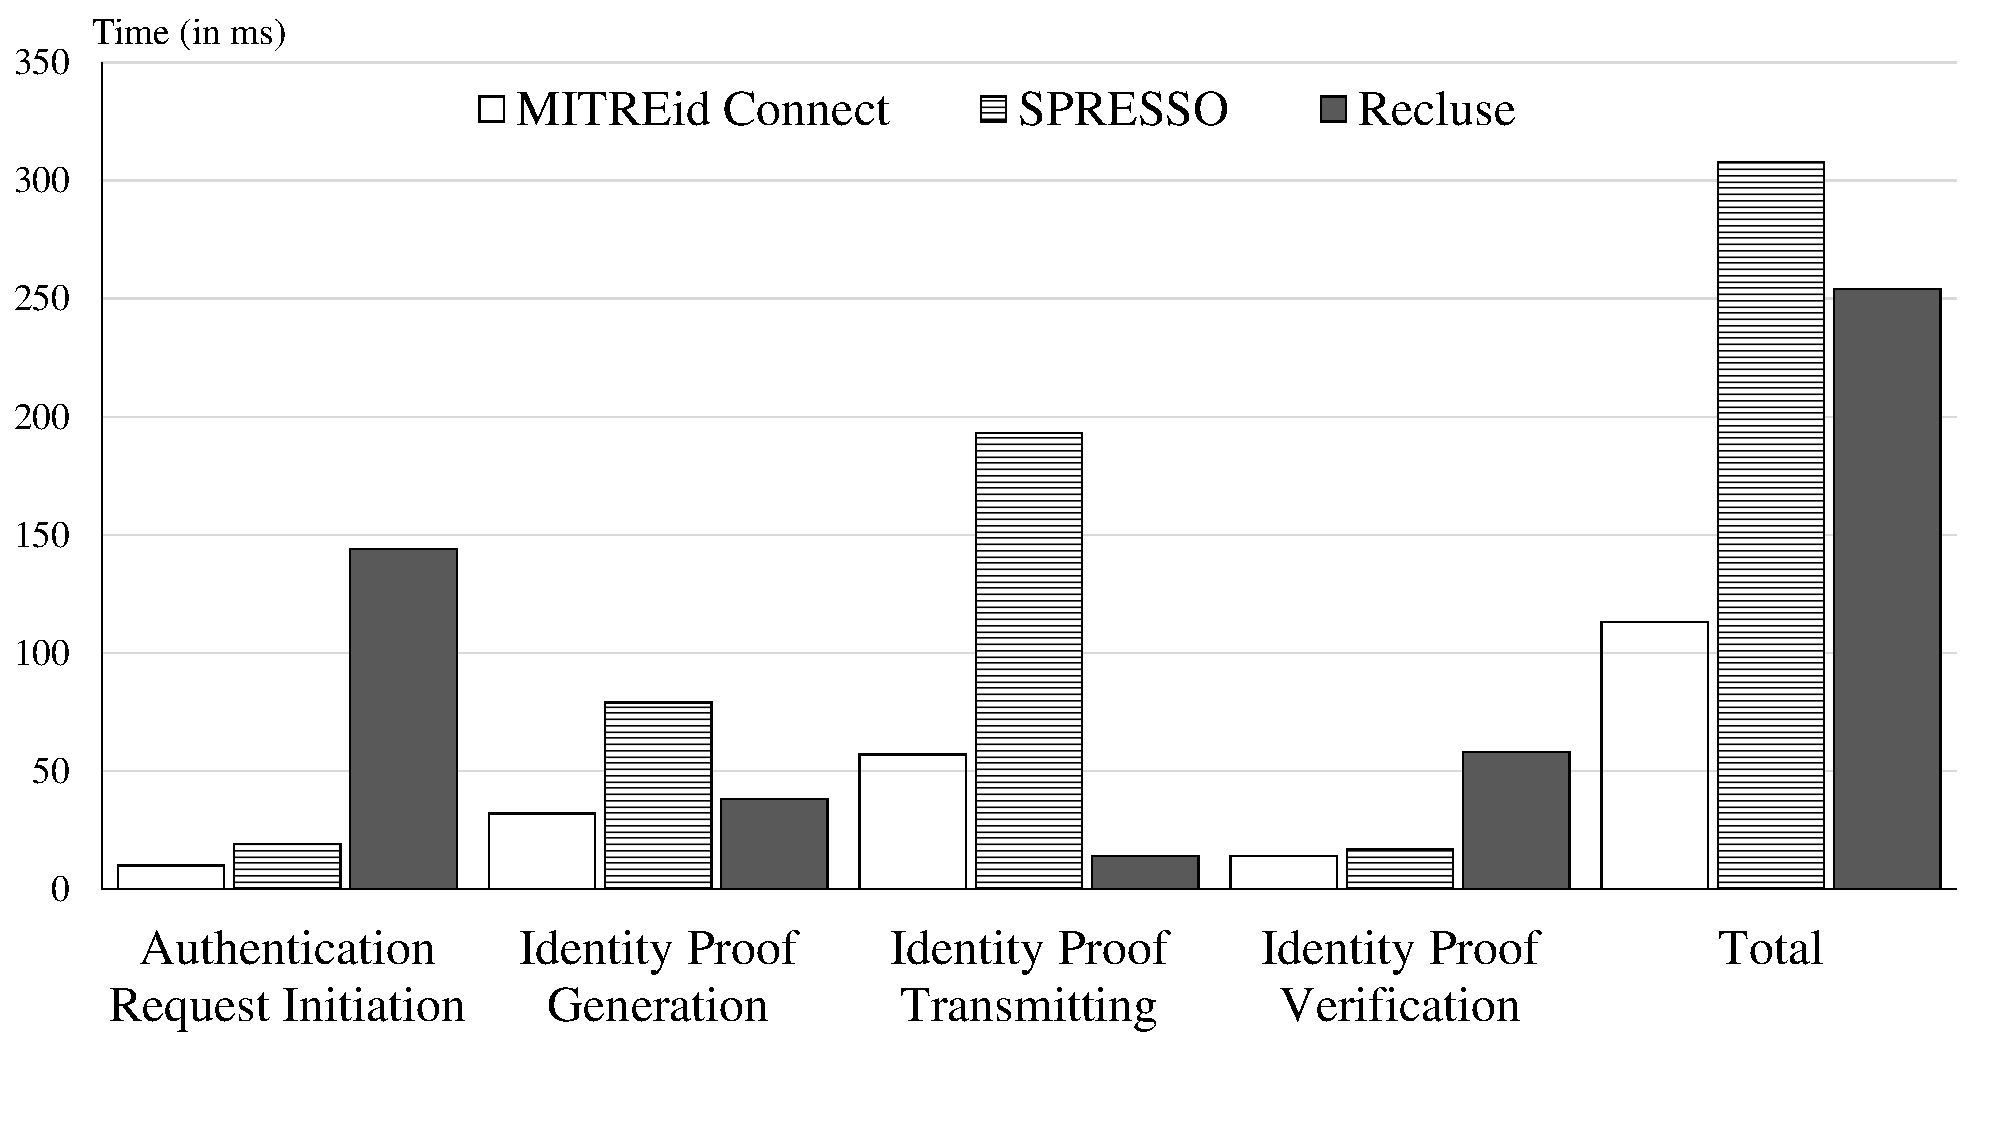
\includegraphics[width=\linewidth]{fig/evaluation2.pdf}
  \caption{The Evaluation.}
  \label{fig:evaluation}
\end{figure}
In the authentication request initiation, MITREid Connect requires the shortest time (10 ms); SPRESSO needs 19 ms for RP to obtain the IdP's public information and encrypt its domain; UPRESSO needs 98 ms, for the $PID_{RP}$ calculation (1 modular exponentiation at the user and 2 at the RP) and RP identifier renewal.

For identity proof generation, MITREid Connect needs 32 ms (information constructing and signing); UPRESSO needs an extra 6 ms for the generation of $PID_U$;  SPRESSO requires 71 ms for a different format of identity proof, which is longer than others as the processing in SPRESSO is implemented with JavaScript while the others are using Java and it costs more time for signature generation by JavaScript because of the programming language feature.

For identity proof transmition, IdP in  MITREid Connect provides the proof as a fragment component (i.e., proof is preceded by \#) to RP to avoid the reload of RP document; and RP uses the JavaScript code to send the proof to the background server; the total transmitting requires 57 ms. In UPRESSO, a chrome extension relays the identity proof from the IdP to RP, which needs 14 ms. The transmitting in SPRESSO is much complicated: The user's browser creates an iframe of the trusted entity (FWD), downloads the JavaScript from FWD, who obtains the RP's correct URL through a systematic decryption and communicates with the parent opener (also RP's document, but avoiding leaking RP to IdP) and RP's document through 3 post messages, which need about 193 ms.
%The time for transmitting identity proof in SPRESSO, relies on the performance of the user's host, 193 ms in our original user, and 127 ms in a stronger user.

In identity proof verification, the RP in MITREid Connect needs 14 ms for verifying the signature, SPRESSO requires 17 ms for a systematic decryption and signature verification, while UPRESSO needs 58 ms for calculation of $Account$ and signature verification.



\begin{comment}
The consideration of usability about UPRESSO is time cost in each authentication. However, the UPRESSO also introduces the extra storage as IdP and RP has to remember the longer identifier of user and RP. But the storage cost is within the range of TBs, which is to be ignored.

In the authentication request initiated phase, MITREid Connect uses the shortest time, 10 ms, as it only builds the request with the stored parameters, such as RP identifier and endpoint. SPRESSO introduces the additional request from RP to IdP for IdP's public parameters and the encryption operation to generate \verb+tag+ (the encrypted RP identifier), so that the time cost is 19 ms. UPRESSO use the longest time, 98 ms , which introduces the extra negotiation and dynamic registration in this phase including 1 time Modular Exponentiation computations at user agent and 2 Modular Exponentiation computations at RP.

In the phase of identity proof generated, all of the systems offer the signed identity proof. Compared with MITREid Connect, UPRESSO only introduces the extra Modular Exponentiation computation for $PPID$. However, the SPRESSO provides the totally different format of identity proof. The time cost in this phase of MITREid Connect, SPRESSO and UPRESSO are 32 ms, 78 ms and 38 ms.

In the phase of identity proof transmitted, UPRESSO transmits the identity proof through the extension and the MITREid Connect uses JavaScript code in RP's web page , the time cost of which are 14 ms and 57 ms. The SPRESSO requires the additional opened iframe, which downloads the script from FWD for extra encryption and decryption operation for identity proof transmitted. However, the time cost of these operations are significant different while running user agent in different devices. We get the 127 ms in average at best, however, in another low-performance device (), the number is 453 ms. To verify whether the performance of user agent has the same influence on UPRESSO, we use several PCs to log in UPRESSO and record the time. The result is the time costs in these PCs are quite similar which means the performance of user agent is not apparently influential with UPRESSO.

The identity proof verified at RP only costs about 1 ms for signature verifying, which is 58 ms at RP requiring additional Modular Exponentiation and Extended Euclidean computation. The RP of SPRESSO has to decrypt the identity proof and verify the signature, which costs 13 ms.

In conclusion, compared with MITREid Connect, UPRESSO introduces about 135 ms extra time cost in authentication request initiated and identity proof verified, which is acceptable. Compared with the best result of SPRESSO, UPRESSO still saves 85 ms.
\end{comment}



